\section{Proposed Method: ASCENSION}
\label{sec:method}

In this section, we propose ASCENSION, a new DA framework for
TSC. We first identify why
in-distribution generative augmentation underperforms across
diverse datasets (Section~\ref{sec:method:motivation}). We then
describe the three ingredients that allow ASCENSION to address
this failure mode: a VAE backbone
(Section~\ref{sec:method:vae}), a contrastive clustering
constraint that keeps classes compact and separated
(Section~\ref{sec:method:contrastive}), and an $\alpha$-scaling
mechanism that expands each class's latent density into
under-represented neighbourhoods
(Section~\ref{sec:method:alpha}).

\subsection{Why in-distribution generative augmentation underperforms}
\label{sec:method:motivation}

Existing generative DA methods for TSC
learn to model the training distribution faithfully, but by
design, rarely produce samples that extend beyond its empirical
support. When the test distribution drifts away from training (through sample scarcity, distributional shift, or class
regions that the encoder under-represents), augmentation
strictly within the empirical support cannot supply the
classifier with examples near the parts of the decision
boundary that matter most. 
ASCENSION follows directly from this observation. Rather than
mimicking the training posterior, we propose expanding
 it in a controlled, class-aware manner so that augmented
samples are more likely to populate the under-represented latent neighbourhoods of
each class. However, expanding the empirical support is
geometrically precarious: naive scaling pushes samples across
class boundaries, causing label-flipping. Safe expansion
therefore requires an explicit geometric account of these
boundaries, which we formalise through a variance decomposition
in Section~\ref{sec:method:alpha}.


\subsection{VAE backbone and training objective}
\label{sec:method:vae}\label{sec:method:contrastive}

ASCENSION adopts a VAE architecture for its ability to flexibly
capture the data distribution in a learned latent space. Given a
labelled dataset $\mathcal{D} = \{(x_i, y_i)\}_{i=1}^{N}$ with
$y_i \in \{1, \ldots, Y\}$, we denote by
$\mathcal{Z} \subseteq \mathbb{R}^{d_z}$ the $d_z$-dimensional
latent space. The encoder defines an approximate posterior
$q_\phi(z \mid x) = \mathcal{N}\bigl(z;\,\mu_\phi(x),\,\Sigma_\phi(x)\bigr)$
over $\mathcal{Z}$, with diagonal covariance
$\Sigma_\phi(x) = \mathrm{diag}\bigl(\sigma_\phi(x)^{2}\bigr)$
(where $\sigma_\phi(x)$ is the encoder's standard-deviation
vector),
and the decoder $p_\theta(x \mid z)$ defines a likelihood under
the prior $p(z) = \mathcal{N}(0, I_{d_z})$.
% ADDED FOR TMLR (rebuttal C6)
Concretely, both networks are fully connected. The encoder
applies two layers of width 1000 with ReLU activations, followed
by separate linear heads for the posterior mean and log-variance
in a $d_z = 50$-dimensional latent space, and the decoder maps
the latent code back to the input length through one layer of
width 1000 with a tanh output.
We deliberately avoid
class conditioning (cVAE), which can amplify posterior collapse
when $x$ is highly correlated with $y$
\citep{dang2023posteriorcollapse}; an empirical comparison with
cVAE baselines is reported in
% REVISED FOR TMLR (rebuttal C6)
Appendix~\ref{app:cvae_baseline}, where the cVAE baselines use
the identical backbone with the one-hot label concatenated to
both the encoder and the decoder inputs. To encourage class-discriminative
geometry, we additionally attach an auxiliary classifier head
$h_\psi : \mathcal{Z} \to \mathbb{R}^{Y}$ on the latent code,
trained jointly with the VAE.

\paragraph{Training objective.}
ASCENSION is trained by minimising a weighted sum of four terms,
\begin{equation}
\mathcal{L}_{\text{VAE}}
= \underbrace{\gamma_1\,\mathcal{L}_{\text{recon}}
            + \gamma_2\,\mathcal{L}_{\text{KL}}}_{\text{negative ELBO}}
+ \underbrace{\gamma_3\,\mathcal{L}_{\text{cluster}}}_{\text{contrastive clustering}}
+ \underbrace{\gamma_4\,\mathcal{L}_{\text{class}}}_{\text{auxiliary classifier}},
\label{eq:total-loss}
\end{equation}
with non-negative weights $\gamma_i$. The first two terms are
the standard ELBO components: a reconstruction loss
$\mathcal{L}_{\text{recon}} = \|x - \mu_\theta(z)\|_{2}^{2}$, where $\mu_\theta(z)$ is the decoder mean,
and a Kullback-Leibler (KL) divergence
$\mathcal{L}_{\text{KL}} =
D_{\mathrm{KL}}\!\bigl(q_\phi(z\mid x) \,\|\, p(z)\bigr)$ that
regularises the posterior toward the prior. The third term is
the margin-based contrastive loss of \citet{hadsell2006contrastive},
applied here to the per-sample posterior means
$z_i = \mu_\phi(x_i)$,
\begin{equation}
\mathcal{L}_{\text{cluster}}
= \frac{1}{N^{2}} \sum_{i,j}
  \mathbf{1}_{y_i = y_j}\, d_{ij}^{2}
+ \mathbf{1}_{y_i \neq y_j}\, \max(0, m - d_{ij})^{2},
\quad d_{ij} = \|z_i - z_j\|_{2},
\label{eq:cluster}
\end{equation}
which pulls same-class means together and pushes different-class
means apart by at least the margin $m > 0$. The fourth term is
the cross-entropy between the auxiliary classifier $h_\psi$ and
the labels,
\begin{equation}
\mathcal{L}_{\text{class}}
= -\frac{1}{N}\sum_{i=1}^{N}
  \log \mathrm{softmax}\bigl(h_\psi(z_i)\bigr)_{y_i},
\quad z_i \sim q_\phi(z \mid x_i),
\label{eq:class}
\end{equation}
 The
contrastive loss shapes the inter-class geometry of posterior means,
while the classifier head extends this discriminative pressure to
the per-sample posterior; together they produce the latent geometry
that Section~\ref{sec:method:alpha} exploits.

\subsection{Latent class expansion}
\label{sec:method:alpha}

The goal of ASCENSION's augmentation step is to expand each
class's latent distribution into under-represented
neighbourhoods while preserving class identity. We define (i) an $\alpha$-scaled class
density that controls within-class spread, and  (ii) a Bayes region
that the rejection step uses to enforce class consistency.

\begin{definition}[$\alpha$-scaled class density]
\label{def:alpha-density}
For class $y \in \{1,\ldots,Y\}$, let
$\mathcal{I}_y = \{i : y_i = y\}$ index the training samples
with label $y$. The \emph{$\alpha$-scaled class density} is the
uniform mixture of encoder posteriors with covariance scaled by
$\alpha \geq 1$:
\begin{equation}
d_y^{\,\alpha}(z)
= \frac{1}{|\mathcal{I}_y|}
  \sum_{i \in \mathcal{I}_y}
    \mathcal{N}\!\bigl(z;\,\mu_\phi(x_i),\,\alpha\,\Sigma_\phi(x_i)\bigr).
\label{eq:alpha-density}
\end{equation}
\end{definition}

\begin{definition}[Bayes region]
\label{def:bayes-region}
For class $y$ and $\alpha \geq 1$,
\begin{equation}
\mathcal{R}_y^{\,\alpha}
= \bigl\{\,z \in \mathcal{Z} :
  y = \arg\max\nolimits_{y' \in \{1,\ldots,Y\}}
       d_{y'}^{\,\alpha}(z)\bigr\}.
\end{equation}
$\mathcal{R}_y^{\,\alpha}$ is the latent region where
$d_y^{\,\alpha}$ dominates the other class mixture densities,
equivalently the maximum-a-posteriori region under a uniform
class prior.
\end{definition}

\paragraph{Why both ingredients are required.}
The $\alpha$-scaling and contrastive losses are not independent
levers: they interact through the geometry of the Bayes
region. Proposition~\ref{prop:variance} makes this precise by decomposing
the variance of the sampling density.

\begin{proposition}[Variance decomposition of $d_y^{\,\alpha}$]
\label{prop:variance}
Let $\bar\mu_y \;\coloneqq\; \tfrac{1}{|\mathcal{I}_y|}
\sum_{i\in\mathcal{I}_y}\mu_\phi(x_i)$ denote the empirical
mean of the per-sample posterior means in class $y$.
For any $\alpha \geq 0$,
\begin{equation}
\mathrm{Cov}_{Z \sim d_y^{\,\alpha}}\!\bigl[Z\bigr]
\;=\;
\alpha\,
\underbrace{
\frac{1}{|\mathcal{I}_y|}\sum_{i\in\mathcal{I}_y}\Sigma_\phi(x_i)
}_{\displaystyle \bar\Sigma_w(y)\;\text{\itshape\small (within-class spread)}}
\;+\;
\underbrace{
\frac{1}{|\mathcal{I}_y|}\sum_{i\in\mathcal{I}_y}
\bigl(\mu_\phi(x_i)-\bar\mu_y\bigr)\bigl(\mu_\phi(x_i)-\bar\mu_y\bigr)^{\!\top}
}_{\displaystyle \Sigma_b(y)\;\text{\itshape\small (between-class spread)}}.
\label{eq:var-decomp}
\end{equation}
The proof is deferred to
Appendix~\ref{app:variance-proof}.
\end{proposition}

\begin{figure}[!t]
\begin{minipage}[t]{0.54\textwidth}
\vspace{0pt}
Figure~\ref{fig:prop1-heatmap} shows the ratio
$m/\sigma_w$ on its $y$-axis, where $m$ is the inter-class
centroid distance enforced by $\mathcal{L}_{\text{cluster}}$
and $\sigma_w = \sqrt{\lambda_{\max}(\bar\Sigma_w(y))}$ is the
within-class radius along the most-spread principal direction
of $\bar\Sigma_w(y)$ ($\lambda_{\max}$ denotes the largest
eigenvalue). We plot this ratio rather than $m$ alone because
the absolute scale of the latent space depends on encoder
hyperparameters. In practice $\sigma_w \approx 1$ (the $\mathcal{N}(0, I)$ prior pulls the
posterior toward unit variance).

\paragraph{Augmentation procedure.}
With the geometry in place, augmentation reduces to sampling
from $d_y^{\,\alpha}$ and rejecting candidates that fall outside
$\mathcal{R}_y^{\,\alpha}$. At each iteration, the VAE is first
trained using $\mathcal{L}_{\text{VAE}}$
(Eq.~\ref{eq:total-loss}) on the current dataset.
% REVISED FOR TMLR (rebuttal Q2)
We then draw $|\mathcal{I}_y|$ candidate latent points from
$d_y^{\,\alpha}$ for each class $y$, one per real sample of the
class and $n$ in total across classes, and keep only the
candidates that lie in the source class's
$\mathcal{R}_y^{\,\alpha}$ (the maximum a posteriori rule
under a uniform class prior), so each iteration adds at most
$n$ synthetic samples.
Accepted candidates are decoded through $p_\theta(x \mid z)$
and folded into the training set; the loop iterates by
retraining the model from scratch on the augmented dataset.
% ADDED FOR TMLR (rebuttal Q3)
Each iteration re-estimates the class mixtures $d_y^{\,\alpha}$
on the already-augmented data, so the expansion compounds in
small steps that the Bayes-region filter keeps in-class.
The full procedure is given in
Algorithm~\ref{alg:ascension}.
\end{minipage}
\hfill
\begin{minipage}[t]{0.44\textwidth}
\vspace{0pt}
\centering
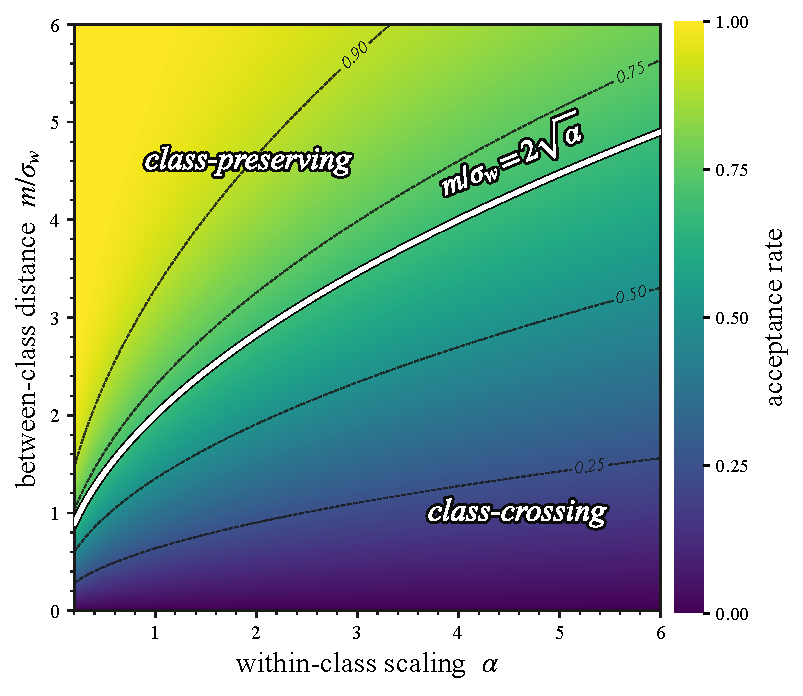
\includegraphics[width=\linewidth]{figures/fig_prop1_heatmap.pdf}
\caption{Acceptance landscape under
Proposition~\ref{prop:variance}. The colour shows
$\mathbb{P}_{Z\sim d_y^{\,\alpha}}\!\bigl[Z\in\mathcal{R}_y^{\,\alpha}\bigr]$
on the $(\alpha, m/\sigma_w)$ plane.
Bold curve $m/\sigma_w = 2\sqrt{\alpha}$ traces where the
$\alpha$-scaled within-class spread $\sqrt{\alpha}\,\sigma_w$
equals the half-distance $m/2$ to the nearest neighbour.}
\label{fig:prop1-heatmap}
\end{minipage}
\end{figure}

Equation~\ref{eq:var-decomp} attributes the spread of
$d_y^{\,\alpha}$ to two distinct sources: encoder noise scaled
by $\alpha$ (first term) and the within-class dispersion of
posterior means (second term, $\alpha$-independent). The
contrastive loss $\mathcal{L}_{\text{cluster}}$ shapes both:
its same-class component drives $\Sigma_b(y)$ small (each class
collapses to a tight cluster of posterior means). Its
different-class component pushes centroids of distinct classes
apart by an inter-class margin $m$ (not appearing in Equation~\ref{eq:var-decomp} but still
constraining the layout around $\mathcal{R}_y^{\,\alpha}$).

Without $\mathcal{L}_{\text{cluster}}$, $m \to 0$ and any
$\alpha$-inflated sample crosses into a neighbouring Bayes region. Therefore,
the rejection step in Algorithm~\ref{alg:ascension} discards
almost all candidates and the $\alpha$-mechanism degenerates to
noise. Figure~\ref{fig:prop1-heatmap} visualises the resulting
acceptance landscape, and the ablation in
Section~\ref{sec:analysis:ablation} (\tablename~\ref{tab:ablation})
confirms the prediction empirically: removing
$\mathcal{L}_{\text{cluster}}$ collapses the mean augmentation
gain to near zero across the 102 UCR datasets.



\begin{algorithm}[H]
  \caption{ASCENSION augmentation loop}
  \label{alg:ascension}
  \begin{algorithmic}[1]
    \Require Original TS data
      $\mathbf{X} = \{x_1, \ldots, x_n\}$ with labels
      $\mathbf{Y} = \{y_1, \ldots, y_n\}$
    \Ensure Augmented datasets
      $\mathbf{X}_{\text{aug}}, \mathbf{Y}_{\text{aug}}$
    \State $\mathbf{X}_{\text{aug}} \gets \mathbf{X}$,\;
           $\mathbf{Y}_{\text{aug}} \gets \mathbf{Y}$
    \While{augmentation desired}
      \State $\theta^{*}, \phi^{*} \gets
              \arg\min_{\theta,\phi}
                \mathcal{L}_{\text{VAE}}$
                using $(\mathbf{X}_{\text{aug}}, \mathbf{Y}_{\text{aug}})$
      \For{\textbf{all} classes $y$}
        % REVISED FOR TMLR (rebuttal Q2)
        \State Sample $|\mathcal{I}_y|$ candidates
          $\mathbf{Z}_{\text{new}}^{y} \sim d_y^{\,\alpha}$,
          one per real sample of class $y$
          \Comment{Definition~\ref{def:alpha-density}}
        \State $\mathbf{Z}_{\text{accept}}^{y} \gets
          \{\,z' \in \mathbf{Z}_{\text{new}}^{y}
          : z' \in \mathcal{R}_y^{\,\alpha}\,\}$
          \Comment{Definition~\ref{def:bayes-region}}
        \State Decode
          $x' = \mu_{\theta^{*}}(z')$ for all
          $z' \in \mathbf{Z}_{\text{accept}}^{y}$
      \EndFor
      \State Append decoded $(x', y)$ pairs to
        $(\mathbf{X}_{\text{aug}}, \mathbf{Y}_{\text{aug}})$
    \EndWhile
  \end{algorithmic}
\end{algorithm}

% -----------------------------------------------------------------
% NOTE — the discussion of cVAE baselines previously sat here as
% §3.5 ("Why not a class-conditional VAE?"). Moved to the appendix
% for TMLR resubmission to keep §3 focused on the method itself.
% Discussion now lives in Appendix~\ref{app:cvae_baseline}; the
% comparison table is in Section~\ref{sec:results:cvae}.
% -----------------------------------------------------------------
